\documentclass{beamer}
\usecolortheme{wolverine}

% math stuff
\usepackage{amsmath}
\usepackage{amsthm}
\usepackage{amssymb}
\usepackage{xcolor}

\usepackage{float}
\usepackage{subcaption}

% to insert images
\usepackage{graphicx}

% to correctly insert stressed characters
\usepackage[T1]{fontenc}
\usepackage[utf8]{inputenc}

\usepackage{multirow}

% Bibliography
% \usepackage[style=alphabetic]{biblatex}
% \usepackage[nottoc]{tocbibind}
% \usepackage{bibentry}
% \setcounter{biburllcpenalty}{9000}
% \usepackage{nameref}
% \addbibresource{slides.bib}

% to put links in table of contents
\usepackage{hyperref}
\hypersetup{colorlinks=false, %set true if you want colored links
	linktoc=all,     %set to all if you
}

\usepackage{mathtools}

% Add symbols
% \usepackage{textcomp}

% Add command for Real and Z sets
% \usepackage{dsfont}
% \newcommand{\Rset}{$\mathds{R}$}
% \newcommand{\Zset}{$\mathds{Z}$}

% Code highlighting
% \usepackage{minted}
% \usemintedstyle{perldoc}
% \setminted{
%     frame=single,
%     breaklines,
% }

% tikz figures
% \usepackage{tikzit}
% \input{style.tikzstyles}

% number rounding
\usepackage{siunitx}
\sisetup{round-mode=places,round-precision=5}

\definecolor{myyellow}{RGB}{225, 225, 0}

\title{Thesis notes}
\date{13th April}

% any code between @(...)@ is escaped back to LaTeX
% \lstset{escapeinside={@(}{)@}}

% algorithms
\usepackage[ruled,vlined]{algorithm2e}

\newtheorem{theorem}{Theorem}

\begin{document}
\frame{\titlepage}

\begin{frame}[c]
	\frametitle{The Echo Chamber Problem - notation}
	\begin{itemize}
		\item $G = (V, E ^{+}, E ^{-}) $ interaction graph
		\item $ \mathcal{C} $ set of contents
		\item $C \in \mathcal{C} $ content, $\mathcal{T} _{C} $ set of threads
		      associated with $C$. A thread $T \in \mathcal{T} _{C} $ is a
		      subgraph of $G$
		      % So $G = \bigcup _{C
		      % \in \mathcal{C} } \bigcup _{T \in \mathcal{T} _C} T $ union of all
		      % threads of all contents
		\item $U \subseteq V$ subset of users, $T[U]$ subgraph of $T$ induced
		      by $U$. $|T(U)|$ is the number of edges of this subgraph
	\end{itemize}
\end{frame}

\begin{frame}[c]
	\frametitle{The Echo Chamber Problem - notation}
	\begin{itemize}
		\item $\eta(C)$ fraction of negative edges associated with $C$
		      (analogous definition for a thread $T$). Content (or thread)
		      controversial if $\eta \in [\alpha, 1]$
		\item $\hat{\mathcal{C} } \subseteq \mathcal{C} $ set of \textit{controversial}
		      contents

		\item $\mathcal{S} _C (U)$ set of \textit{non controversial} threads
		      induced by $U$, for \textit{controversial} contents, i.e.

			      {\small
				      \begin{equation}
					      \mathcal{S} _{C} (U) = \{ T[U] \; s.t. \; T[U] \; non \;
					      controversial, T \in \mathcal{T} _{C}, C
					      \in \hat{\mathcal{C}}, U \subseteq V\}
				      \end{equation}
			      }
	\end{itemize}

\end{frame}

\begin{frame}[c]
	\frametitle{The Echo Chamber Problem}
	\textbf{Goal}: given an interaction graph $G$, find $U \subseteq V$ maximing

	\begin{equation}
		\xi (U) = \sum^{}_{C \in \hat{\mathcal{C}} } \sum^{}_{T[U] \in S_C (U)}
		| T[U] |
	\end{equation}

	The set of users maximing the expression is denoted as $\hat{U}$ and the
	corresponding score is $\xi(G)$
\end{frame}

\begin{frame}[c]
	\frametitle{Computing exactly the score}

	\begin{equation}
		maximize\; \sum_{ij \in E(T_{k}), T_{k} \in \mathcal{T}_{C}, C \in
			\mathcal{\hat{C}} } x_{ij} ^{k}
	\end{equation}
	\begin{equation}
		x _{ij}^{k}  \leq y_i, \; x _{ij} ^{k} \leq y_j, \;x _{ij}^{k}  \leq z_k \quad\quad \forall ij \in E(T_{k}), T_{k} \in
		\mathcal{T}_{C}, C \in \mathcal{\hat{C}}
	\end{equation}
	\begin{equation}
		x _{ij} ^{k} \geq - 2 + y_i + y_j + z_k \quad\quad \forall ij \in E(T_k), T_k \in \mathcal{T} _{C}, C \in \hat{\mathcal{C} }
	\end{equation}
	\begin{equation}
		\sum^{}_{ij \in E^{-} (T_k)} x_{ij}^{k}  - \alpha \sum^{}_{ij \in E(T_k)}
		x_{ij} ^{k}  \leq - \alpha z_k \quad\quad \forall T_{k} \in \mathcal{T} _{C}, C \in
		\hat{\mathcal{C}}
	\end{equation}
	\begin{equation}
		y _{i} \in  \{0, 1\} \quad\quad \forall i \in V
	\end{equation}
	\begin{equation}
		0 \leq x _{ij} ^{k}  \leq 1 \quad\quad \forall ij \in E(T_{k}), T_{k} \in
		\mathcal{T}_{C}, C \in \mathcal{\hat{C}}
	\end{equation}
	\begin{equation}
		0 \leq z _{k} \leq 1 \quad\quad \forall T_{k} \in \mathcal{T} _{C}, C \in
		\hat{\mathcal{C}}
	\end{equation}
\end{frame}

\begin{frame}[c]
	\frametitle{The Densest Echo Chamber Problem}
	\textbf{Goal}: given an interaction graph $G$, find $U \subseteq V$ maximing

	\begin{equation}
		\psi (U) = \sum^{}_{C \in \hat{\mathcal{C}} } \sum^{}_{T[U] \in S_C (U)}
		\frac{| T[U] |}{|U|}
	\end{equation}

	The set of users maximing the expression is denoted as $\hat{U}$ and the
	corresponding score is $\psi(G)$
\end{frame}

\begin{frame}[c]
	\frametitle{Echo Chamber Problem inapproximability}
	\begin{theorem}
		\label{th:approximability}
		Echo Chamber Problem (ECP) has no $n^{1-\epsilon} $-approximation algorithm for
		any $\epsilon$ unless $\mathcal{P} = \mathcal{NP}  $
	\end{theorem}

	\begin{theorem}
		\label{th:approximability}
		Densest Echo Chamber Problem (D-ECP) has no $n^{1-\epsilon} $-approximation algorithm for
		any $\epsilon$ unless $\mathcal{P} = \mathcal{NP}  $
	\end{theorem}
\end{frame}

\begin{frame}[c]
	\frametitle{Solving exactly the D-ECP}

	\begin{equation}
		maximize\; \sum_{ij \in E(T_{k}), T_{k} \in \mathcal{T}_{C}, C \in
			\mathcal{\hat{C}} } x_{ij} ^{k}
	\end{equation}
	\begin{equation}
		x _{ij}^{k}  \leq y_i, \quad x _{ij} ^{k} \leq y_j \quad\quad \forall ij \in E(T_{k}), T_{k} \in
		\mathcal{T}_{C}, C \in \mathcal{\hat{C}}
	\end{equation}
	\begin{equation}
		a _{ij} ^{k} \geq - 2 + b_i + b_j + z_k , \quad z_k \geq a_{ij}^{k}  \quad\quad \forall ij \in E(T_k), T_k \in \mathcal{T} _{C}, C \in \hat{\mathcal{C} }
	\end{equation}
	\begin{equation}
		\sum^{}_{ij \in E^{-} (T_k)} a_{ij}^{k}  - \alpha \sum^{}_{ij \in E(T_k)}
		a_{ij} ^{k}  \leq - \alpha z_k \quad\quad \forall T_{k} \in \mathcal{T} _{C}, C \in
		\hat{\mathcal{C}}
	\end{equation}
	\begin{equation}
		\sum^{}_{i \in V} y_i \leq 1
	\end{equation}
	\begin{equation}
		y _{i} \geq 0, \quad b _{i} \in \{0, 1\},
		\quad b_i \geq y_i\quad\quad \forall i \in V
	\end{equation}
	\begin{equation}
		x _{ij} ^{k}  \geq 0, \quad a _{ij} ^{k}  \in \{0, 1\}, \quad a_{ij}
			^{k} \geq x_{ij} ^{k}  \quad\quad \forall ij \in E(T_{k}), T_{k} \in
		\mathcal{T}_{C}, C \in \mathcal{\hat{C}}
	\end{equation}
	\begin{equation}
		0 \leq z _{k} \leq 1 \quad\quad \forall T_{k} \in \mathcal{T} _{C}, C \in
		\hat{\mathcal{C}}
	\end{equation}
\end{frame}

\begin{frame}[c]
	\frametitle{Computing exactly the score}
	$y_{i} > 0 \implies b_i = 1$ means that $y_i \in U$.

	$z_k = 1$ means that thread $k$ is non controversial.

	$x_{ij}^{k}  > 0 \implies a_{ij}^{k} = 1 $ means that the edge contributes to the score.

	\bigskip

	The following constraints enforce that only edges $ij$ whose both vertices
	are in $U$ and are associated to a non controversial thread can contribute.
	Also if one edge contributes to the score $\implies $ thread is not
	controversial.

	\begin{equation*}
		x _{ij}^k \leq y_i \quad \forall ij \in E(\hat{\mathcal{C}})
	\end{equation*}
	\begin{equation*}
		x _{ij}^{k}  \leq y_j \quad \forall ij \in E(\hat{\mathcal{C}})
	\end{equation*}
	\begin{equation*}
		a _{ij} ^{k} \leq z_k \quad \forall ij \in E(T_k), T_k \in \mathcal{T} _{C}, C \in \hat{\mathcal{C} }
	\end{equation*}

\end{frame}

\begin{frame}[c]
	\frametitle{Computing exactly the score}
	Also, considering edges contributing to the score, they must not produce a
	controversial thread

	\begin{equation*}
		\sum^{}_{ij \in E^{-} (T_k)} a_{ij}^{k}  - \alpha \sum^{}_{ij \in E(T_k)}
		a_{ij}^k \leq - \alpha z_{k}  \quad \forall T_{k} \in \mathcal{T} _{C}, C \in
		\hat{\mathcal{C}}
	\end{equation*}

	If $T_{k} [U]$ is controversial, then $x_{ij} $ must be $0 \; \forall ij \in
		E(T_{k}[U] )$.

	\bigskip

	In general either all $ij \in E(T_{k}[U] )$ are $0$ or they are $1$.

	\begin{equation*}
		a _{ij}^{k}  \leq z_k \quad \forall ij \in E(T_k), T_k \in \mathcal{T} _{C}, C \in \hat{\mathcal{C} }
	\end{equation*}
	\begin{equation*}
		a _{ij} ^{k} \geq - 2 + b_i + b_j + z_k \quad \forall ij \in E(T_k), T_k \in \mathcal{T} _{C}, C \in \hat{\mathcal{C} }
	\end{equation*}
\end{frame}

\begin{frame}[c]
	\frametitle{Computing exactly the score}
	Density introduced by

	\begin{equation*}
		\sum^{}_{i \in V} y_i \leq 1
	\end{equation*}

	\begin{figure}[htpb]
		\centering
		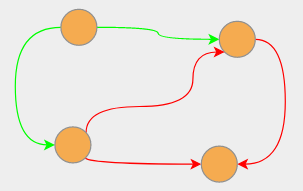
\includegraphics[width=0.3\linewidth]{img/graph-example2-1.png}
	\end{figure}
\end{frame}

\begin{frame}[c]
	\frametitle{The datasets - negative edge fractions for contents}
	\begin{figure}
		\begin{center}
			\begin{subfigure}[b]{0.4\textwidth}
				\centering
				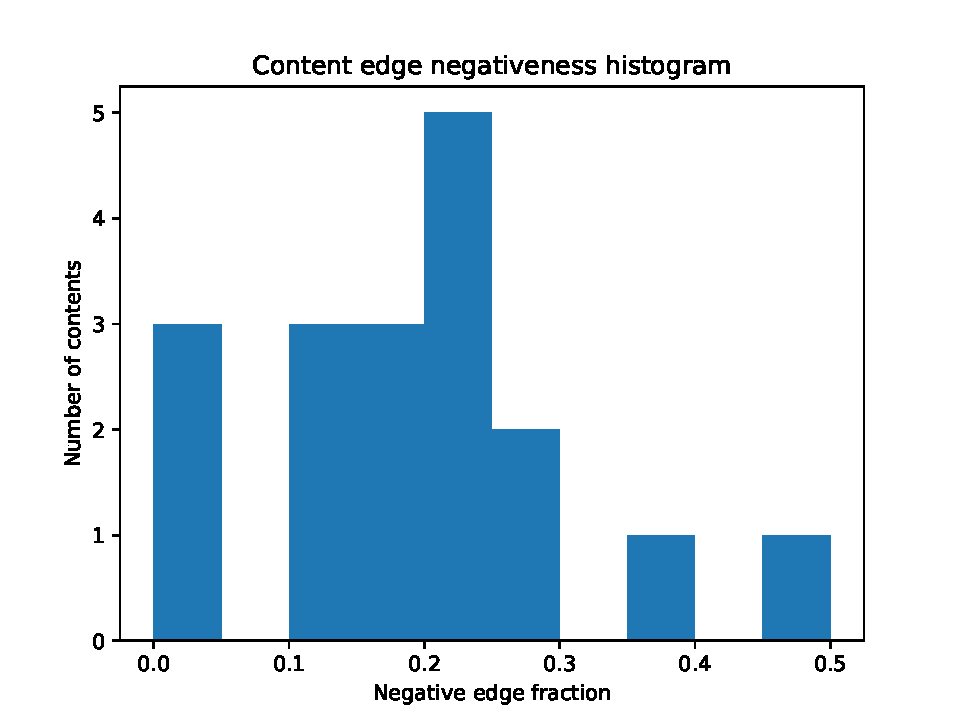
\includegraphics[width=\textwidth]{out/emanews200/neg-fraction-content-hist.pdf}
				\caption{@emanews}
				\label{fig:out/emanews200/neg-fraction-content-hist.pdf}
			\end{subfigure}
			\begin{subfigure}[b]{0.4\textwidth}
				\centering
				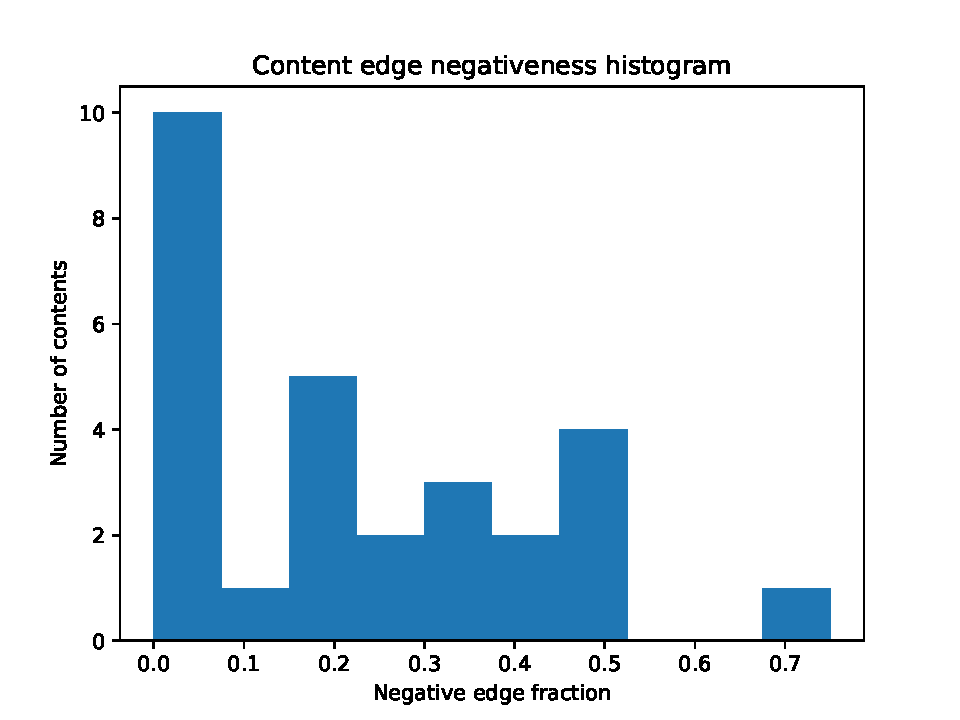
\includegraphics[width=\textwidth]{out/bbcscience200/neg-fraction-content-hist.pdf}
				\caption{@bbcscience}
				\label{fig:out/bbcscience200/neg-fraction-content-hist.pdf}
			\end{subfigure}
			\begin{subfigure}[b]{0.4\textwidth}
				\centering
				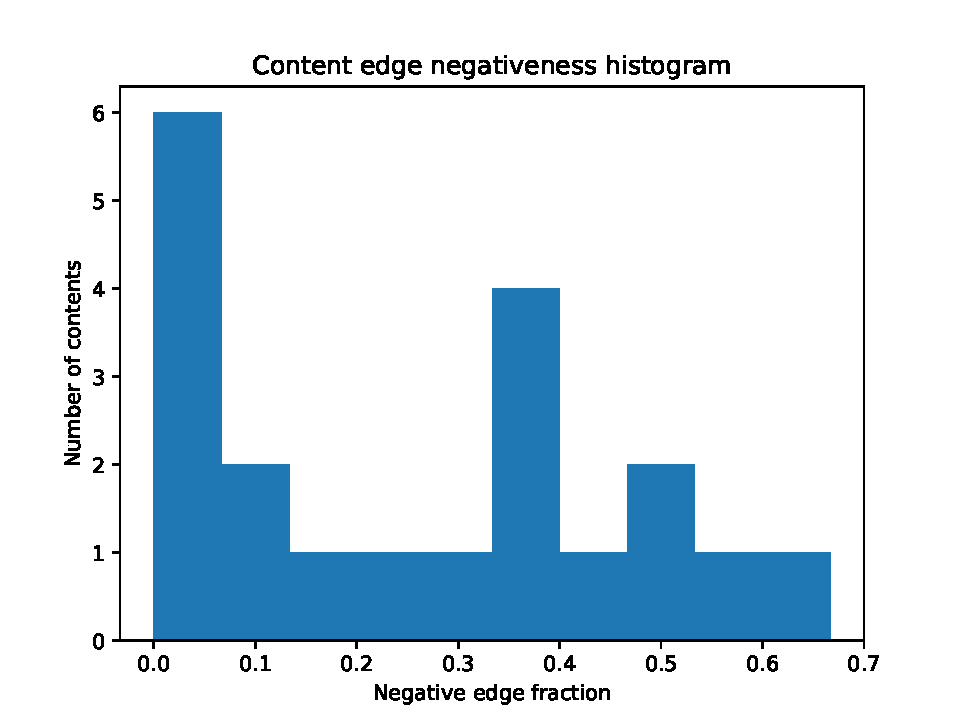
\includegraphics[width=\textwidth]{out/bbcentertainment200/neg-fraction-content-hist.pdf}
				\caption{@bbcentertainment}
				\label{fig:out/bbcscience200/neg-fraction-content-hist.pdf}
			\end{subfigure}
			\begin{subfigure}[b]{0.4\textwidth}
				\centering
				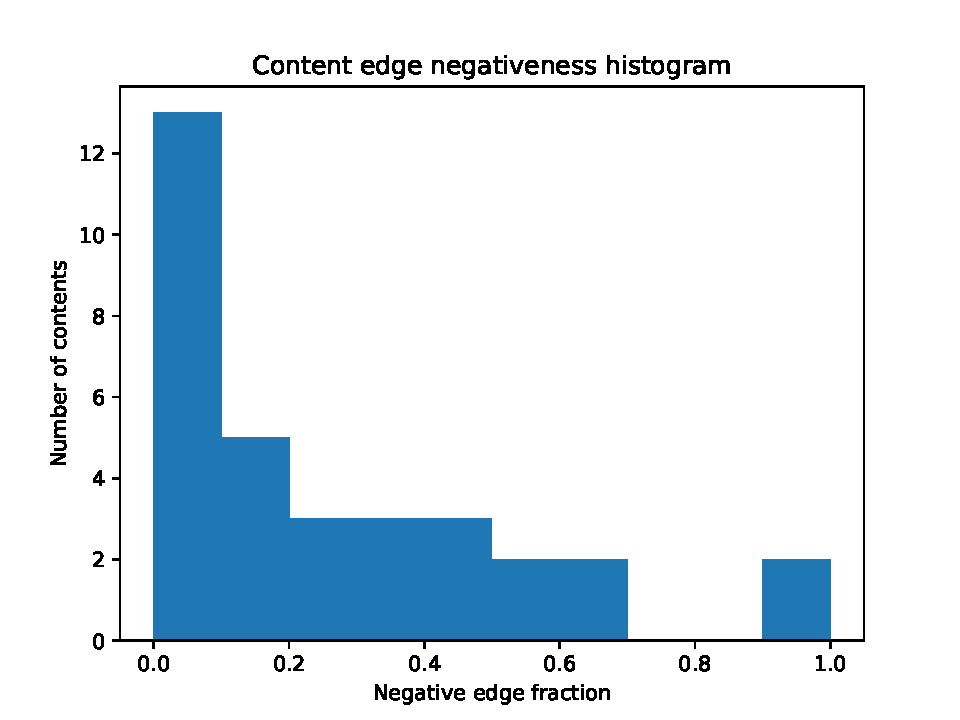
\includegraphics[width=\textwidth]{out/bbctech200/neg-fraction-content-hist.pdf}
				\caption{@bbctech}
				\label{fig:out/emanews200/neg-fraction-content-hist.pdf}
			\end{subfigure}
		\end{center}
	\end{figure}

\end{frame}


\begin{frame}[c]
	\frametitle{An initial implementation - results}
	\begin{itemize}
		\item Beta algorithm was repeated $ \sqrt{n}$ times for a graph with $n$ nodes
	\end{itemize}

	\begin{table}[htpb]
		\centering
		\caption{Echo chamber scores, greedy approach}
		\begin{tabular}{c|c|c|c|c}
			\textbf{Source}     & {|V|}                   & {|E|}
			                    & $(\xi_\beta(G), \beta)$ &
			$\xi_{peel} (G)$                                                       \\
			\hline
			{@emanews}          & {1226}                  & {1842} & (0, *)    & 0 \\
			{@bbcscience}       & {477}                   & {388}  & (3, 0.9)  & 7 \\
			{@bbcentertainment} & {220}                   & {183}  & (21, 1.0)
			                    & 16                                               \\
			{@bbctech}          & {793}                   & {719}  & (101, *)
			                    & 107                                              \\
		\end{tabular}
	\end{table}
	\begin{table}[htpb]
		\centering
		\caption{Echo chamber scores, MIP approaches}
		\begin{tabular}{c|c|c|c}
			\textbf{Source}     & $\xi_{MIP}(G) $ & $\xi_{MIPr}(G)$ &
			$\xi_{MIPr\_alg}(G)$                                          \\
			\hline
			{@emanews}          & 0               & 1.43            & 0   \\
			{@bbcscience}       & 7               & 10.76           & 7   \\
			{@bbcentertainment} & 34              & 41.69           & 34  \\
			{@bbctech}          & 309             & 326.63          & 309 \\
		\end{tabular}
	\end{table}
\end{frame}

\begin{frame}[c]
	\frametitle{An initial implementation - timings}
	\begin{itemize}
		\item Timings are reported in seconds.
	\end{itemize}

	\begin{table}[htpb]
		\centering
		\caption{Echo chamber timings, greedy approach}
		\begin{tabular}{c|c|c|c|c}
			\textbf{Source}     & {|V|}  & {|E|}  & Beta & Peeling \\
			\hline

			{@emanews}          & {1226} & {1842} & 0.5  & 18062   \\
			{@bbcscience}       & {477}  & {388}  & 0.05 & 678     \\
			{@bbcentertainment} & {220}  & {183}  & 0.1
			                    & 81                               \\
			{@bbctech}          & {793}  & {719}  & 80
			                    & 4031                             \\
		\end{tabular} \end{table}
	\begin{table}[htpb]
		\centering
		\caption{Echo chamber timings, MIP approaches}
		\begin{tabular}{c|c|c|c}
			\textbf{Source}     & MIP  & MIP relaxation &
			MIP relaxation alg                                 \\
			\hline
			{@emanews}          & 3.77 & 0.08           & 2.8  \\
			{@bbcscience}       & 0.82 & 0.07           & 0.26 \\
			{@bbcentertainment} & 0.79 & 0.09           & 1.04 \\
			{@bbctech}          & 2.39 & 0.38           & 1.76 \\
		\end{tabular}
	\end{table}
\end{frame}
\end{document}
